\documentclass[11pt,a4paper]{article}

\usepackage[margin=0.8in]{geometry}
\usepackage{graphicx}
\usepackage{amsmath,amssymb}
\usepackage{booktabs}
\usepackage{float}
\usepackage{microtype}
\usepackage[hidelinks]{hyperref}
\usepackage{array}
\usepackage{xcolor}

\title{Large Language Models\\
Homework 2}
\author{Chia-Hsuan Hsu \quad Student ID: 315511079}
\date{Fall 2026}

\begin{document}

\maketitle

% ============================================================
% Problem 1
% ============================================================

\section{Selective Memory with State-Space Models}

\subsection{Setup}

Each prompt is a sequence of 6--30 four-token records followed by
\texttt{QUERY K ANSWER}. Two to four records are \texttt{STORE K V}
with distinct keys, and the others are \texttt{NOISE K V}, which must be
ignored even if they reuse a stored key. The model reads the
representation at the final valid position (the \texttt{ANSWER} token)
and predicts one of the 32 values V0--V31. The course splits are used
without modification: 12,000 training, 1,500 validation, and 2,000 test
prompts. Only \texttt{train.jsonl} is used for optimisation and only
\texttt{val.jsonl} for model selection.

Questions 1--3 use the prescribed backbone: an embedding, two causal
SSM blocks $x \leftarrow x+\mathrm{Dropout}(\mathrm{GELU}(\mathrm{SSM}(\mathrm{LN}(x))))$,
a final LayerNorm and a 32-way head, with $d=N=64$, dropout 0.1, AdamW
(learning rate $10^{-3}$, weight decay 0.01), batch size 64, 10 epochs,
gradient clipping 1.0, and seed 42. Both models use the same
initialisation rule for their shared parameter types:
$a=\sigma(\theta_a)$ evenly spaced over $[0.5,0.99]$,
$B,C,D,W_g\sim\mathcal{N}(0,1/\text{fan-in})$, and gate bias $b_g=0$.
No prescribed setting was changed for Questions 1--3.

% ------------------------------------------------------------

\subsection{Basic Diagonal SSM (Q1)}

\paragraph{Implementation.}
For an input $x\in\mathbb{R}^{B\times L\times d}$ the block computes
$u_t=Bx_t\in\mathbb{R}^{B\times L\times N}$, the state
\[
h_t=a\odot h_{t-1}+Bx_t,\qquad h_0=0,
\]
and the output $y_t=Ch_t+Dx_t\in\mathbb{R}^{B\times L\times d}$, with
no biases in $B$, $C$, $D$. The recurrence is evaluated with a parallel
(Hillis--Steele) prefix scan over time: in $\lceil\log_2 L\rceil$ rounds
each position $t$ is combined with position $t-2^k$, using only
products of decays in $(0,1)$, so it is numerically stable. The scan is
exactly the sequential recurrence (maximum difference from a literal
loop of the equations: $1.1\times10^{-6}$) and strictly causal
(changing tokens after position 10 leaves all outputs up to position 10
unchanged). The state is never stored on the module, so every forward
pass starts from $h_0=0$ for each sample and each layer. With right
padding, all \texttt{PAD} tokens come after \texttt{ANSWER}; by
causality they cannot affect it, and the model reads index
$\texttt{lengths}-1$ rather than the last padded column. A padded and an
unpadded copy of the same prompt give the same prediction.

\paragraph{Results.}
The best validation accuracy is \textbf{0.1913 at epoch 10} (validation
loss 2.858). Training loss falls almost linearly from 3.49 to 2.73 and
validation loss from 3.45 to 2.86, and validation accuracy still rises
every epoch (Figure~\ref{fig:p1-curves}, left). The gap between the two
losses is small, so the basic model is clearly \emph{under}-fitted, not
over-fitted. With a fixed decay $a$, every record (STORE or NOISE) is
written with the same weight and old STORE values decay exponentially,
so the model has no mechanism to keep only the valid pairs.

\begin{figure}[H]
    \centering
    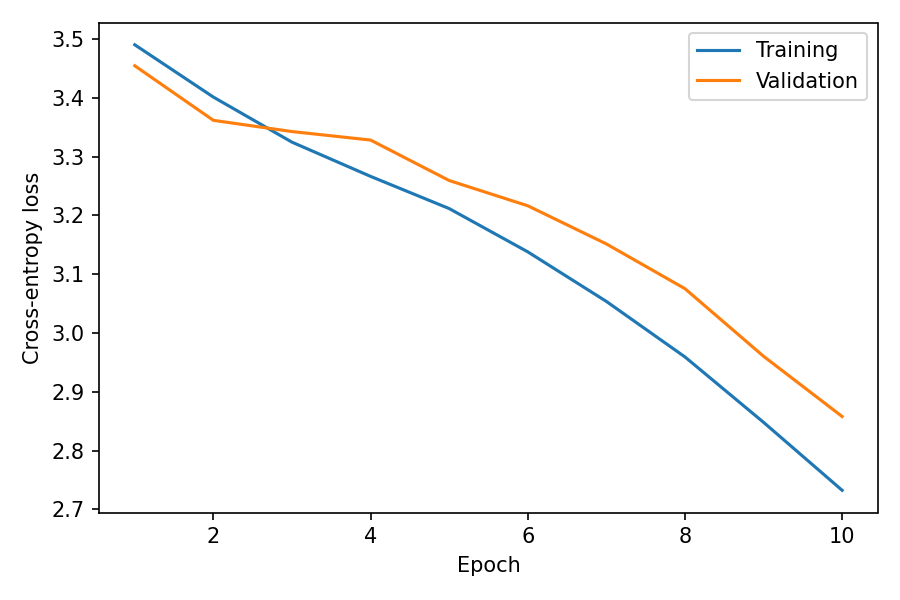
\includegraphics[width=0.49\linewidth]{p1_basic_curves.png}\hfill
    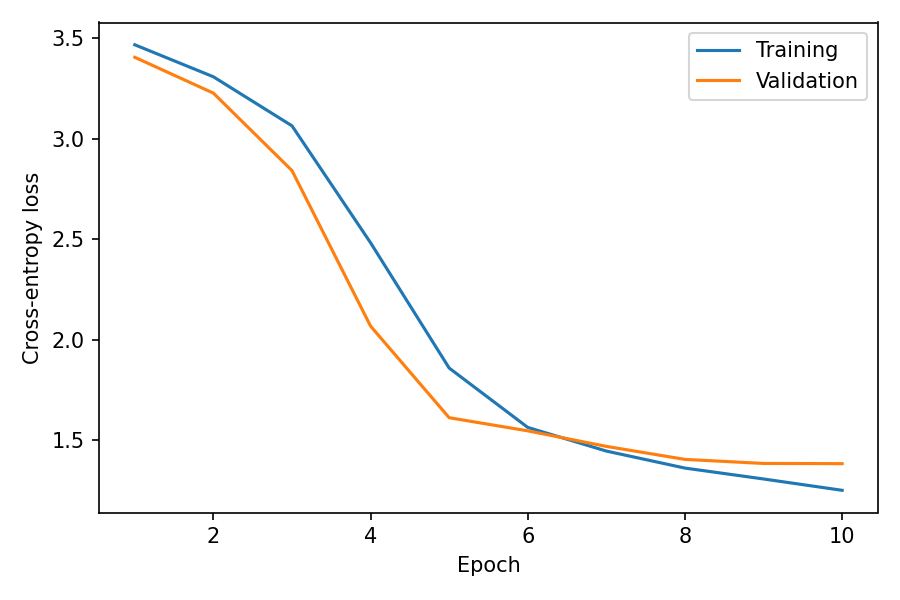
\includegraphics[width=0.49\linewidth]{p1_gated_curves.png}
    \caption{Training and validation cross-entropy of the basic SSM
    (left) and the gated SSM (right) under identical settings.}
    \label{fig:p1-curves}
\end{figure}

% ------------------------------------------------------------

\subsection{Input-Gated SSM (Q2)}

\paragraph{Implementation.}
The gate is computed from the LayerNorm-ed current input,
$g_t=\sigma(W_gx_t+b_g)\in(0,1)^N$. The candidate is
$\tilde h_t=a\odot h_{t-1}+Bx_t$, and the new state is
$h_t=(1-g_t)\odot h_{t-1}+g_t\odot\tilde h_t$. This is algebraically the
linear recurrence
\[
h_t=\bigl(1-g_t\odot(1-a)\bigr)\odot h_{t-1}+g_t\odot Bx_t,
\]
so the same parallel scan is used with a time-varying decay
$\lambda_t=1-g_t(1-a)$ (maximum difference from a literal loop of the
PDF equations: $9.5\times10^{-7}$). When $g_t\approx0$, the channel
ignores the current token and copies its state unchanged, without any
decay. When $g_t\approx1$, it performs the full basic update; with a
small $a$ this overwrites the channel. The gate therefore lets the model
decide, token by token, what to write and what to keep.

\paragraph{Results.}
The best validation accuracy is \textbf{0.4060 at epoch 8} (validation
loss 1.404), more than twice the basic model under the same settings.
The curves (Figure~\ref{fig:p1-curves}, right) drop quickly between
epochs 3 and 5 (validation accuracy 0.19 $\rightarrow$ 0.39) and then
flatten at 0.37--0.41. The training loss (1.25) and validation loss
(1.38) stay close, so over-fitting is at most mild.

The failure cases explain the plateau. The gated model almost always
predicts a value that \emph{was stored}, so it has learned to ignore
NOISE records, but it often returns the value of a \emph{different}
STORE key. Guessing uniformly among the 2--4 stored values gives
$(1/2+1/3+1/4)/3\approx0.36$, very close to the observed 0.39--0.41.
Gating solves the ``ignore noise'' part of the task, but the small model
has not learned to \emph{bind} each value to its key.

% ------------------------------------------------------------

\subsection{Performance and Cost Comparison (Q3)}

\begin{table}[H]
    \centering
    \caption{Comparison of the selected checkpoints (NVIDIA
    A100-SXM4-40GB, FP32, batch size 64).}
    \label{tab:p1-cost}
    \begin{tabular}{lcc}
        \toprule
        Metric & Basic SSM & Gated SSM\\
        \midrule
        Trainable parameters & 31,712 & 40,032\\
        Validation accuracy & 0.1913 (epoch 10) & \textbf{0.4060} (epoch 8)\\
        Training time (seconds/epoch) & \textbf{2.24} & 2.47\\
        Inference throughput (samples/s) & \textbf{30,696} & 27,129\\
        Peak GPU allocated memory (MiB) & \textbf{92.5} & 104.8\\
        \bottomrule
    \end{tabular}
\end{table}

\paragraph{Measurement.}
Both models are trained by the same script on the same GPU, in FP32,
with batch size 64 and the same data order (seed 42). Training time is
the mean over epochs of the training loop only, with
\texttt{torch.cuda.synchronize()} before the timer starts and before it
stops; validation and plotting are excluded. Throughput uses the
selected checkpoint in \texttt{eval()} mode under \texttt{no\_grad}, on
the first validation batch (64 prompts, padded to length 124) already on
the GPU: 3 warm-up forward passes, then 10 timed passes between two
synchronisations. Peak memory is \texttt{torch.cuda.max\_memory\_allocated}
during training.

\paragraph{Discussion.}
The gated model has 26\% more parameters (an extra $W_g$ and $b_g$ per
layer) and one more matrix product and sigmoid per layer. It is about
10\% slower per epoch, has 12\% lower throughput, and uses 13\% more
memory, because the gate tensor $g\in\mathbb{R}^{B\times L\times N}$
must be stored for back-propagation. In exchange it more than doubles
validation accuracy, so it is the better accuracy--cost trade-off.
Possible reasons for the accuracy difference are:
(1) the \emph{mechanism}: the input-dependent gate can skip NOISE
records and hold stored information without decay;
(2) the \emph{parameter count}: part of the gain may come from extra
capacity rather than from gating itself;
(3) \emph{training randomness and budget}: one seed and only 10 epochs.
The basic model is still improving at epoch 10, and the gated model's
accuracy fluctuates between 0.37 and 0.41 after epoch 5, so differences
of a few points are within run-to-run noise. Runtime differences are
also partly kernel-launch overhead, which dominates for tensors this
small.

\paragraph{Representative failure cases.}
\begin{itemize}
    \item \texttt{val\_000001} (query K20, gold V19): the prompt also
          contains \texttt{NOISE K20 V17}. The basic model predicts V29
          and the gated model predicts V21; neither outputs the noise
          value, so the error is in retrieval rather than in noise
          filtering.
    \item \texttt{val\_000002} (query K23, gold V23, four STORE
          records): the gated model predicts V17, the value of
          \texttt{STORE K16 V17}.
    \item \texttt{val\_000003} (query K1, gold V17): the basic model
          predicts V15, the value of \texttt{STORE K9 V15}.
    \item \texttt{val\_000006} (query K5, gold V21, two
          \texttt{NOISE K5} distractors): the gated model ignores both
          noise values but predicts V4, the value of \texttt{STORE K7 V4}.
\end{itemize}

% ------------------------------------------------------------

\subsection{Improvement and Kaggle Competition (Q4)}

\paragraph{Changes.}
All Q4 models keep the prescribed \texttt{GatedDiagonalSSM} update
equations, use only token inputs, are trained only on
\texttt{train.jsonl}, and stay below $10^6$ trainable parameters.
\begin{enumerate}
    \item \textbf{Task-consistent augmentation of \texttt{train.jsonl}},
          re-drawn every time a sample is loaded: consistent random
          renaming of all keys (a permutation of K0--K31) and all values
          (a permutation of V0--V31, with the label mapped too), random
          shuffling of the record order (the task states that order is
          random), and a re-sampled query among the valid STORE keys with
          the recomputed label. Every original and augmented training
          sample is checked: the format is valid, STORE keys are distinct,
          and the label is the STORE value of the query key.
    \item \textbf{Wider state and residual stream}: $d=N=256$ with three
          gated SSM blocks (model D), and $d=192$, $N=256$ with four
          blocks (model E).
    \item \textbf{Prediction head} that combines the final
          \texttt{ANSWER} representation $r$ with the embedding $e_q$ of
          the observed query key:
          $\text{logits}=Wr+b+W_3\bigl((W_1r)\odot(W_2e_q)\bigr)$.
    \item \textbf{Training schedule}: up to 200 epochs, batch size 128,
          AdamW with learning rate $10^{-3}$, 5\% linear warm-up and
          cosine decay, dropout 0, decay initialisation widened to
          $a\in[0.01,0.99]$, an exponential moving average of the weights
          (decay 0.995; still a single model) for validation and
          checkpointing, and early stopping after 40 epochs without
          improvement in validation accuracy.
\end{enumerate}
Model A isolates the effect of augmentation: it is the Q2 model with
augmentation and the new schedule (30 epochs, batch 64).

\paragraph{Why these changes.}
Q2 showed that the bottleneck is binding keys to values. The task needs
a key-addressed \emph{write}, which stores the value of a STORE record
in state associated with its key, and a key-addressed \emph{read} at
the \texttt{ANSWER} position. In the gated SSM, $g_t$ multiplies the
write $Bx_t$, so a state channel can be opened only for ``the value
token of a STORE record whose key is $k$''. The first layer can carry
the record marker and key forward to the value position (open the gate
on the marker or key token, then close it). This gives a multiplicative,
key-selective write, but it needs many state channels (32 keys times a
few channels per value code), hence $N=256$. A residual stream as wide
as the state ($d=256$) lets the final representation carry this memory
to the head, and the element-wise product $(W_1r)\odot(W_2e_q)$ lets the
query key select the matching part of it. Augmentation makes the data
effectively unlimited and forces the model to learn the rule instead of
statistics of particular key or value names.

\begin{table}[H]
    \centering
    \caption{Q4 comparison on \texttt{val.csv} (inference: batch size 64,
    same protocol as Table~\ref{tab:p1-cost}).}
    \label{tab:p1-q4}
    \resizebox{\linewidth}{!}{%
    \begin{tabular}{lcccccc}
        \toprule
        Model & Params & Val acc. & Best epoch & s/epoch & Samples/s & Peak MiB\\
        \midrule
        Gated SSM (Q2) & 40,032 & 0.4060 & 8 & 2.47 & 27,129 & 104.8\\
        A: Q2 + augmentation & 40,032 & 0.4067 & 11 & 3.10 & 27,096 & 105.0\\
        \textbf{D: $d$256, $N$256, 3 layers + query head} & 955,680 & \textbf{0.9913} & 198 & 3.34 & 17,400 & 1041.5\\
        E: $d$192, $N$256, 4 layers + query head & 867,552 & 0.4053 & 13 & 3.72 & 13,230 & 1305.6\\
        \bottomrule
    \end{tabular}}
\end{table}

\begin{figure}[H]
    \centering
    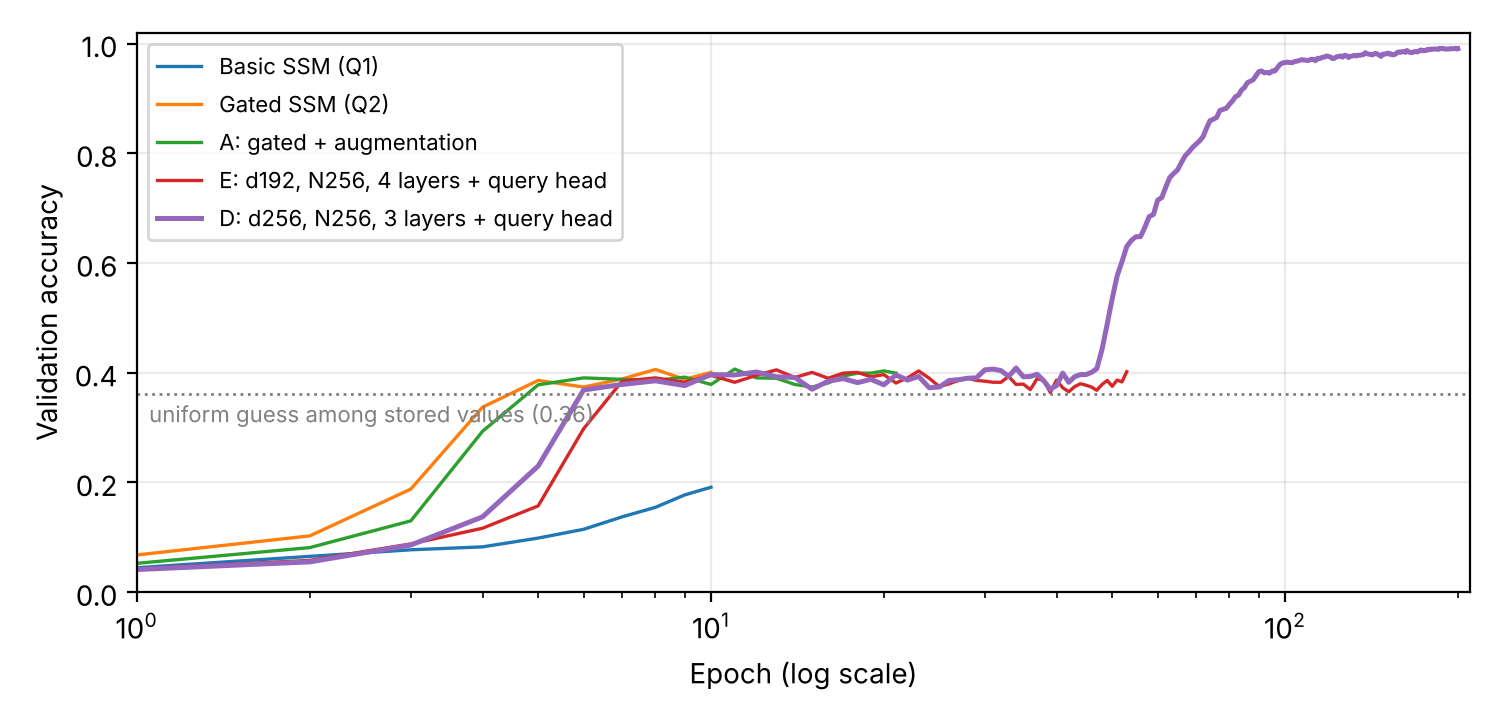
\includegraphics[width=0.9\linewidth]{p1_val_acc.png}
    \caption{Validation accuracy per epoch (log scale). All models first
    reach the $\approx$0.40 plateau of ``a stored value, but not
    necessarily the right one''. Only model D escapes it, around epoch
    48.}
    \label{fig:p1-valacc}
\end{figure}

\begin{figure}[H]
    \centering
    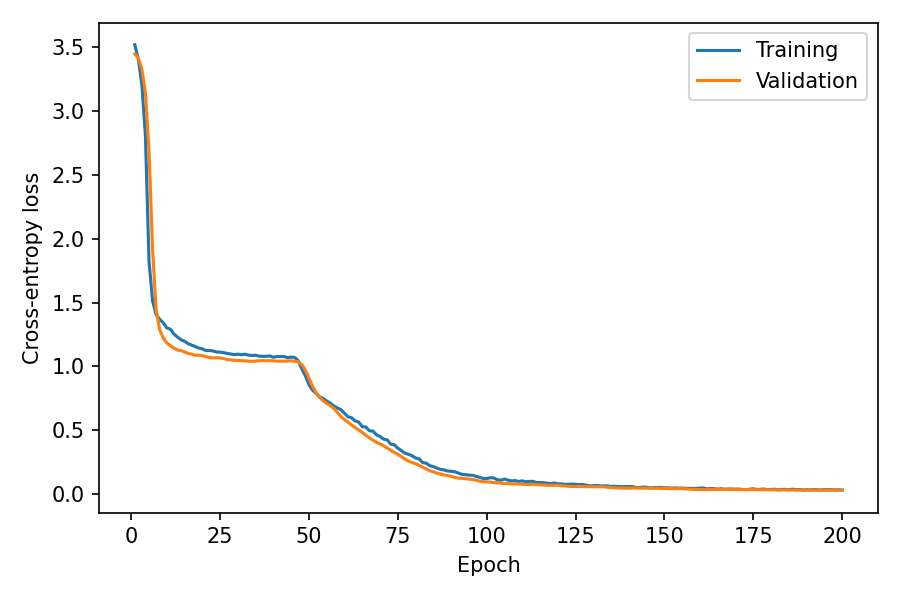
\includegraphics[width=0.6\linewidth]{p1_q4d_curves.png}
    \caption{Training and validation cross-entropy of the final model D.}
    \label{fig:p1-q4d}
\end{figure}

\paragraph{Effect.}
Augmentation alone does not help the small model (A: 0.4067 vs
0.4060), so its bottleneck is capacity and binding, not data. Model D
reaches \textbf{0.9913} validation accuracy, 58.5 points above the
original gated model. The cost is 24$\times$ the parameters (still below
$10^6$), 1.6$\times$ lower inference throughput, and about 10$\times$
the peak training memory. Figure~\ref{fig:p1-valacc} shows that D also
stays on the 0.40 plateau for about 45 epochs; then its accuracy jumps
(0.54 at epoch 50, 0.89 at epoch 80, above 0.98 from epoch 138) as it
discovers the key--value binding. Validation loss falls to 0.030
(Figure~\ref{fig:p1-q4d}), and the best epoch is 198 of 200, so the long
schedule with fresh augmented data was necessary. Model E reached the
same plateau (best 0.4053 at epoch 13) and was stopped by early stopping
at epoch 53. That is only a few epochs after the point where D escaped,
so E's result reflects the patience setting and training randomness at
least as much as its narrower residual stream.

The remaining errors of D (13 of 1,500) are all binding errors on prompts
with three or four STORE records: the prediction is the value of another
stored key. Examples: \texttt{val\_000189} (query K11, gold V28,
predicted V7 from \texttt{STORE K30 V7}) and \texttt{val\_000280} (query
K11, gold V7, predicted V30 from \texttt{STORE K13 V30}). Noise records
are never the source of the error in these cases.

\paragraph{Checkpoint selection and submission.}
Each run saves the epoch with the highest validation accuracy (ties are
broken by lower validation loss), evaluated with the EMA weights. Across
candidates, the run with the highest validation accuracy (D) is selected
automatically. \texttt{test.jsonl} has no labels and is read only once
at the end to write predictions: argmax over V0--V31, columns
\texttt{id,answer}, every test ID exactly once and in the original order
(checked by assertions). Neither validation nor test data is used for
training or augmentation, no ensemble is used, and the public
leaderboard was not used for model selection.

\paragraph{Kaggle.}
Team name: 315511079. Final selected submission:
\texttt{submission (20).csv} from model D, public score
\textbf{0.99500} (Figure~\ref{fig:p1-kaggle}). Both the ordinary
baseline (0.40050) and the strong baseline (0.58350) are exceeded.

\begin{figure}[H]
    \centering
    
\includegraphics[width=0.85\linewidth]{p1_kaggle.png}
    \caption{Final selected Kaggle submission (public score 0.99500).}
    \label{fig:p1-kaggle}
\end{figure}

% ============================================================
% Problem 2
% ============================================================

\section{Masked Diffusion Language Models}

\subsection{Setup}

The provided bidirectional Transformer (6 layers, hidden size 384, 6
heads, input and output embeddings tied, 13,768,704 parameters) is
trained from random initialisation ($\mathcal{N}(0,0.02)$) on the first
120,000 TinyStories training stories. The 8K byte-level BPE tokenizer is
trained on the first 20,000 of them. Stories are split into 128-token
blocks without mixing stories, giving 269,460 training and 2,061
validation blocks (from 1,000 held-out validation stories, never used
for training). Training uses AdamW (learning rate $2\times10^{-4}$,
weight decay 0.05), FP16 autocast with a gradient scaler, gradient
clipping 1.0, batch size 64, and seed 42, on one Google Colab Tesla T4.

Adjustments to the template, all stated in the notebook: 120,000
training stories to match the assignment (the template used 300,000);
batch size 64 instead of 4, which was tuned for a 12\,GB RTX 3060;
training length set to 20 epochs, with a 200-minute cap so that the
whole notebook stays within the 4-hour T4 budget; and a
validation-loss probe every 2,500 steps with a fixed seed, which never
updates the weights.

% ------------------------------------------------------------

\subsection{Implementation (Q1)}

\paragraph{(a) Forward masking.}
For each sequence $t\sim\mathcal{U}(0,1)$ is drawn and clamped to at
least $0.01$; for a fixed ratio the same $t$ is used for the whole
batch. Each position is masked if a uniform random number is below $t$
\emph{and} the token is not \texttt{[PAD]}, so every non-padding token
is masked independently with probability $t$ and padding is never
corrupted. The selected tokens are replaced by \texttt{[MASK]}, and the
function returns $(x_t,\text{mask},t)$ with a Boolean mask. On a
validation block, the measured masked fractions are 0.232, 0.492, and
0.773 for $t=0.25$, $0.50$, and $0.75$.

\paragraph{(b) Loss.}
The model receives $x_t$ and predicts all positions. Token-level
cross-entropy against the clean tokens is computed in FP32, multiplied
by the mask so that only masked positions contribute, summed per
sequence, and divided by $t\cdot L$, where $L$ is that sequence's number
of non-padding tokens:
\[
\mathcal{L}=\frac{1}{B}\sum_{b=1}^{B}\frac{1}{t_bL_b}\sum_{i\in M_b}-\log p_\theta\bigl(x_0^{i}\mid x_t\bigr).
\]
Small $t$ is handled safely: $t\ge0.01$ bounds the weight by $100/L$,
$L$ is clamped to at least 1, and a sequence with no masked token
contributes 0. Since $\mathbb{E}[|M|/(tL)]=1$, the untrained loss should
be close to $\ln|V|$; it is 9.50 versus $\ln 8000=8.99$.

\paragraph{(c) Iterative decoding.}
At each of the $S$ steps the model predicts all positions in parallel,
and \texttt{[PAD]}, \texttt{[MASK]}, and \texttt{[UNK]} are excluded.
The softmax gives a predicted token (argmax) and a confidence (maximum
probability) at each position. Positions that are no longer masked (the
prompt and tokens revealed earlier) get confidence $-\infty$, so only
still-masked positions are ranked. The $k=\lceil\text{remaining}/(S-s)\rceil$
most confident ones are revealed through a Boolean mask and
\texttt{torch.where}; all other tokens stay fixed. A check confirms that
the prompt is unchanged and that no \texttt{[MASK]} is left after the
last step.

% ------------------------------------------------------------

\subsection{Training (Q2)}

\begin{table}[H]
    \centering
    \caption{Training summary.}
    \label{tab:p2-train}
    \begin{tabular}{lc}
        \toprule
        Item & Value\\
        \midrule
        Trainable parameters & 13,768,704 (13.77M)\\
        Optimizer steps & 84,200 (20 epochs $\times$ 4,210 steps)\\
        GPU training time & 112.7 min (Colab Tesla T4)\\
        Final training loss (mean of the last 20 logs) & 2.379\\
        Validation MDLM loss (all 2,061 blocks) & 2.332\\
        Checkpoint & \texttt{outputs/tiny\_mdlm\_v2.pt}\\
        \bottomrule
    \end{tabular}
\end{table}

\begin{figure}[H]
    \centering
    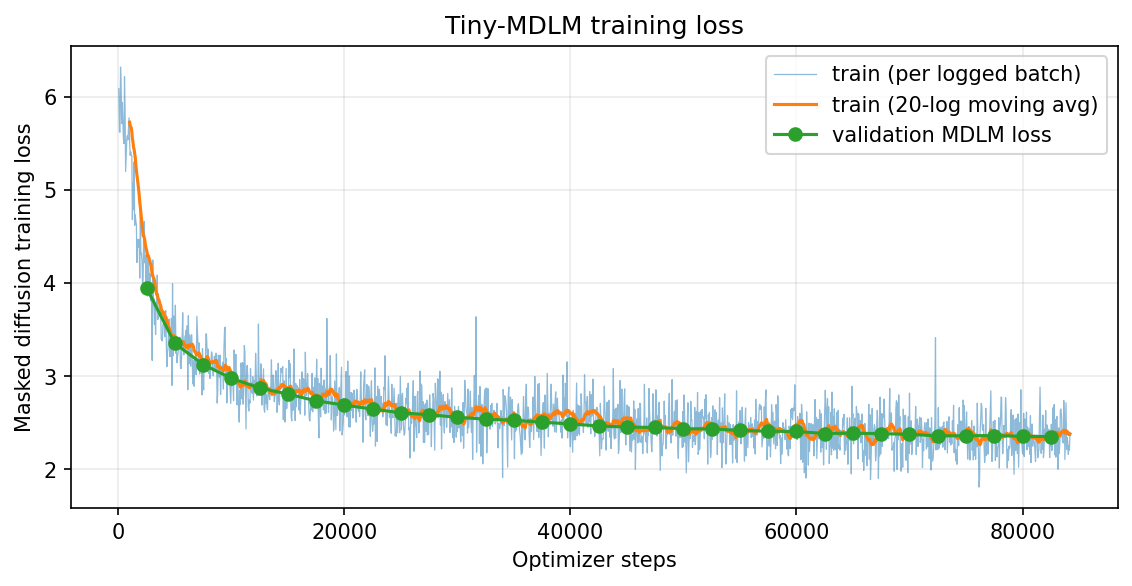
\includegraphics[width=0.9\linewidth]{p2_loss_curve.png}
    \caption{MDLM training loss per logged batch, its moving average,
    and the held-out validation loss (fixed seed).}
    \label{fig:p2-loss}
\end{figure}

The loss decreases clearly (Figure~\ref{fig:p2-loss}). Training loss
falls from about 6 to about 4 in the first 2,500 steps, while the model
learns frequent words, and then slowly to about 2.4. The curve is noisy
because every batch draws new masking ratios, and batches with small
$t$ receive a large $1/t$ weight. Validation loss decreases
monotonically: 3.95 (step 2.5k), 2.87 (12.5k), 2.65 (22.5k), 2.54
(32.5k), 2.47 (42.5k), 2.43 (52.5k), 2.38 (62.5k), 2.36 (72.5k), and
2.35 (82.5k), ending at 2.33. It flattens over the last
$\approx$15k steps but never rises, and the final validation loss is not
higher than the training loss. Over-fitting is therefore not evident
after 20 epochs. Re-masking every block differently in every epoch acts
as strong data augmentation; the flattening suggests that the 14M-parameter
model is approaching its capacity for this budget.

% ------------------------------------------------------------

\subsection{Evaluation and Analysis (Q3)}

\paragraph{(a) Masked cross-entropy.}
MCE is the mean negative log-probability of the original tokens at the
masked positions, measured on all 2,061 validation blocks with fixed-seed
masks. $\exp(\text{MCE})$ is not reported as a perplexity.

\begin{table}[H]
    \centering
    \caption{Validation MCE at fixed masking ratios (lower is better).}
    \label{tab:p2-mce}
    \begin{tabular}{ccc}
        \toprule
        Masking ratio & MCE (nats) & Masked-token accuracy\\
        \midrule
        25\% & 1.160 & 72.2\%\\
        50\% & 1.849 & 59.2\%\\
        75\% & 3.156 & 37.8\%\\
        \bottomrule
    \end{tabular}
\end{table}

\begin{figure}[H]
    \centering
    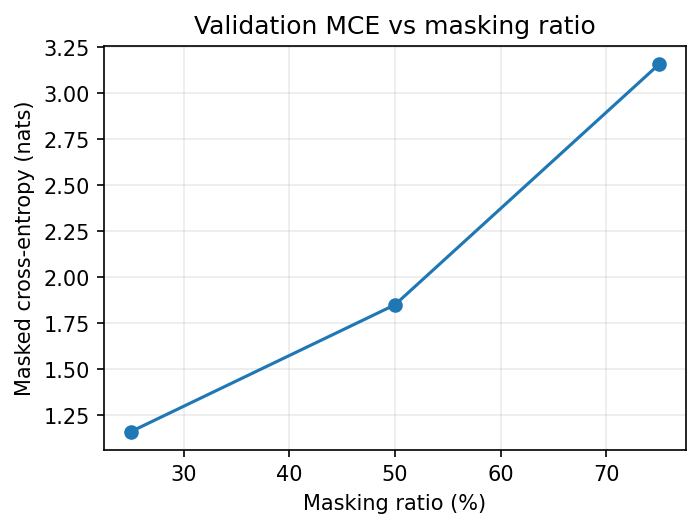
\includegraphics[width=0.5\linewidth]{p2_mce.png}
    \caption{Validation MCE as a function of the masking ratio.}
    \label{fig:p2-mce}
\end{figure}

MCE rises monotonically and faster than linearly with the masking ratio:
+0.69 nats from 25\% to 50\% and +1.31 nats from 50\% to 75\%
(Table~\ref{tab:p2-mce}, Figure~\ref{fig:p2-mce}). With 25\% masking,
most of the context on both sides of a masked token is visible, so the
bidirectional model can often infer it almost deterministically
(function words, punctuation, repeated names such as ``Lily''). With
75\% masking, the remaining context is sparse, many continuations are
plausible, and the prediction approaches an unconditional
language-model guess, so uncertainty is much higher.

\paragraph{(b) Generation.}
Prompt ``Once upon a time'', 64 tokens, greedy confidence-based
unmasking. Times are means of 5 runs after a warm-up, with CUDA
synchronisation.

\begin{table}[H]
    \centering
    \caption{Generations with 4, 8, and 16 decoding steps (distinct-$n$ =
    unique word $n$-grams / all word $n$-grams).}
    \label{tab:p2-gen}
    \small
    \begin{tabular}{c c c p{0.62\linewidth}}
        \toprule
        Steps & Time & distinct-1/2 & Generated text\\
        \midrule
        4 & 14.8\,ms & 0.79 / 0.95 & Once upon a time, there was a little girl named Lily. She loved to play with her her toy bear...,,, she went to school and and saw with..... with the together..... They They played laughed and and and had fun together. The end.\\
        \addlinespace
        8 & 30.3\,ms & 0.77 / 0.98 & Once upon a time, there was a little girl named Lily. She loved to play with her toys and day.. One day, she's mom came in visit room room. She saw Lily playing and and. Lily Lily Lily was happy. She They her back and and played with it together. The end.\\
        \addlinespace
        16 & 61.2\,ms & 0.83 / 1.00 & Once upon a time, there was a little girl named Lily. She loved to play with her toys and especially candy, especially. One One, day Lily's mom told her to be to the park and play more. But Lily was't want to because she she wanted to eat more candy candy. The end.\\
        \bottomrule
    \end{tabular}
\end{table}

\emph{Speed.} Decoding time is almost exactly proportional to the
number of steps (about 3.8\,ms per step), because each step is one full
forward pass over the 64-token sequence.

\emph{Fluency and repetition.} All three settings produce the typical
TinyStories frame (``a little girl named Lily \ldots\ The end.'')
because the first and last tokens are the most predictable and are
revealed first. With 4 steps, about 15 tokens are revealed per step.
They are predicted independently from the same context and cannot
coordinate, which produces punctuation runs (``...,,,'', ``.....''),
adjacent duplicates (``her her'', ``and and and'', ``They They''), and
almost no story content. With 8 steps the text improves (``One day,
she's mom came in visit room''), but repetition remains (``room room'',
``Lily Lily Lily''). With 16 steps the text is the most coherent: it has
a small plot (Lily's mom tells her to go to the park; she wants to eat
more candy), the highest diversity (distinct-1 0.83, distinct-2 1.00),
no punctuation runs, and fewer duplicates (``One One'', ``she she'',
``candy candy''). More steps trade speed for quality, because each token
is conditioned on more already revealed neighbours.

% ------------------------------------------------------------

\subsection{Questions (Q4)}

\paragraph{(a) How does MDLM generation differ from autoregressive
generation?}
An autoregressive model generates strictly left to right, one token per
forward pass, and each token is conditioned only on the prefix through
causal attention, so $n$ tokens need $n$ sequential steps. An MDLM
starts from a fully masked suffix and uses a bidirectional Transformer
to predict all masked positions in parallel. At each step it commits a
subset of them, here the most confident ones, in any order, and later
steps condition on tokens on both sides. The number of steps is a free
speed--quality knob and can be much smaller than the length. In this
sampler, committed tokens are never revised, and tokens revealed in the
same step are chosen independently of each other.

\paragraph{(b) Why are different masking ratios used during training?}
During generation the model must denoise every noise level, from a fully
masked suffix ($t\approx1$) to an almost finished sequence
($t\approx0$). Sampling $t\sim\mathcal{U}(0,1)$ trains one network for
all of these states, and the $1/t$-weighted objective corresponds to the
diffusion ELBO integrated over $t$. It also acts as data augmentation:
the same story yields many different prediction problems, from nearly
unconditional generation to easy cloze filling.

\paragraph{(c) Why might a low reconstruction loss still produce
repetitive or incoherent text?}
The loss measures \emph{per-token marginal} predictions given a context
taken from real data. During generation: (i) many tokens are revealed in
the same step, each from its own marginal, so the joint result can be
inconsistent; for example, two neighbouring positions both choose the
most likely word, which creates repetition such as ``and and and'' in
Table~\ref{tab:p2-gen}. (ii) The model conditions on its own earlier
predictions, which are off the training distribution, so errors
compound. (iii) Greedy maximum-confidence selection favours frequent,
``safe'' tokens (``the'', ``and'', punctuation, names), which creates
loops. (iv) A low MCE is dominated by easy, locally predictable tokens
and says little about global coherence over 64 tokens. More decoding
steps, temperature or top-$p$ sampling, and remasking strategies reduce
these effects.

% ============================================================
% Reproducibility
% ============================================================

\section{Reproducibility}

\begin{table}[H]
    \centering
    \caption{Software and hardware used for the reported runs.}
    \label{tab:env}
    \begin{tabular}{lll}
        \toprule
        & Problem 1 & Problem 2\\
        \midrule
        Platform & Google Colab & Google Colab\\
        GPU & NVIDIA A100-SXM4-40GB & NVIDIA Tesla T4\\
        Python & 3.13.16 & Colab default\\
        PyTorch & 2.11.0+cu130 (CUDA 13.0) & 2.11.0+cu130\\
        Precision & FP32 & FP16 autocast + GradScaler\\
        Seed & 42 & 42\\
        \bottomrule
    \end{tabular}
\end{table}

\clearpage
\paragraph{Procedure.}
\begin{itemize}
    \item \texttt{hw2\_1\_315511079.ipynb}: put \texttt{train.jsonl},
          \texttt{val.jsonl}, and \texttt{test.jsonl} in \texttt{data/}
          (or upload the competition zip) and run all cells. The notebook
          writes \texttt{hw2\_1.py} and \texttt{hw2\_1\_q4.py}, checks the
          SSM implementation against a literal loop, trains Q1/Q2
          (about 25\,s each on an A100) and the Q4 candidates (model D:
          about 3.3\,s per epoch, 200 epochs), selects the final model
          on validation accuracy, writes \texttt{submission.csv}, and
          packs everything into \texttt{hw2\_1\_artifacts.zip}.
    \item \texttt{hw2\_2\_315511079.ipynb}: run all cells on a Colab T4.
          TinyStories is downloaded automatically. Training takes about
          113 minutes, and the last cell packs the checkpoint, tokenizer,
          figures, and \texttt{results.json} into
          \texttt{hw2\_2\_artifacts.zip}.
\end{itemize}
The seed is fixed to 42 in every run. GPU kernels are not forced to be
fully deterministic in Problem 2, so a rerun on different hardware can
change the last digits of the losses. Timing and memory values depend
on the machine.

\paragraph{Note on the saved Problem 2 notebook.}
The training cell prints about 1,700 log lines. In the saved notebook,
its output stops at step 64,700 and the later cells show no output,
because the notebook was saved while training was still running. The
run completed (84,200 steps), and every Problem 2 number in this report
comes from \texttt{results.json} and the figures written by the last
cell of that same run (\texttt{hw2\_2\_artifacts.zip}). The same
numbers and figures are also included in the written report at the end
of the notebook.

\end{document}
